  {\large \fontB Description:}
  
  {\bf solI} is a 2-dimensional analytical solution to the Cauchy equations with the acceleration term set to zero
  to represent creeping flow. The boundary conditions are free-slip everywhere on a unit domain. 
  The viscosity varies exponentially in the z direction.
  The flow is driven by a density jump in the x direction.

 {\large \fontB Parameters:}
  
 The variable parameters of this solution are:
 \begin{itemize}
   \item{density parameter: $ \sigma $.}
   \item{viscosity parameter: $B$.}
   \item{width of dense column: $x_c$.}
 \end{itemize}

  \begin{SCfigure}[][h]
    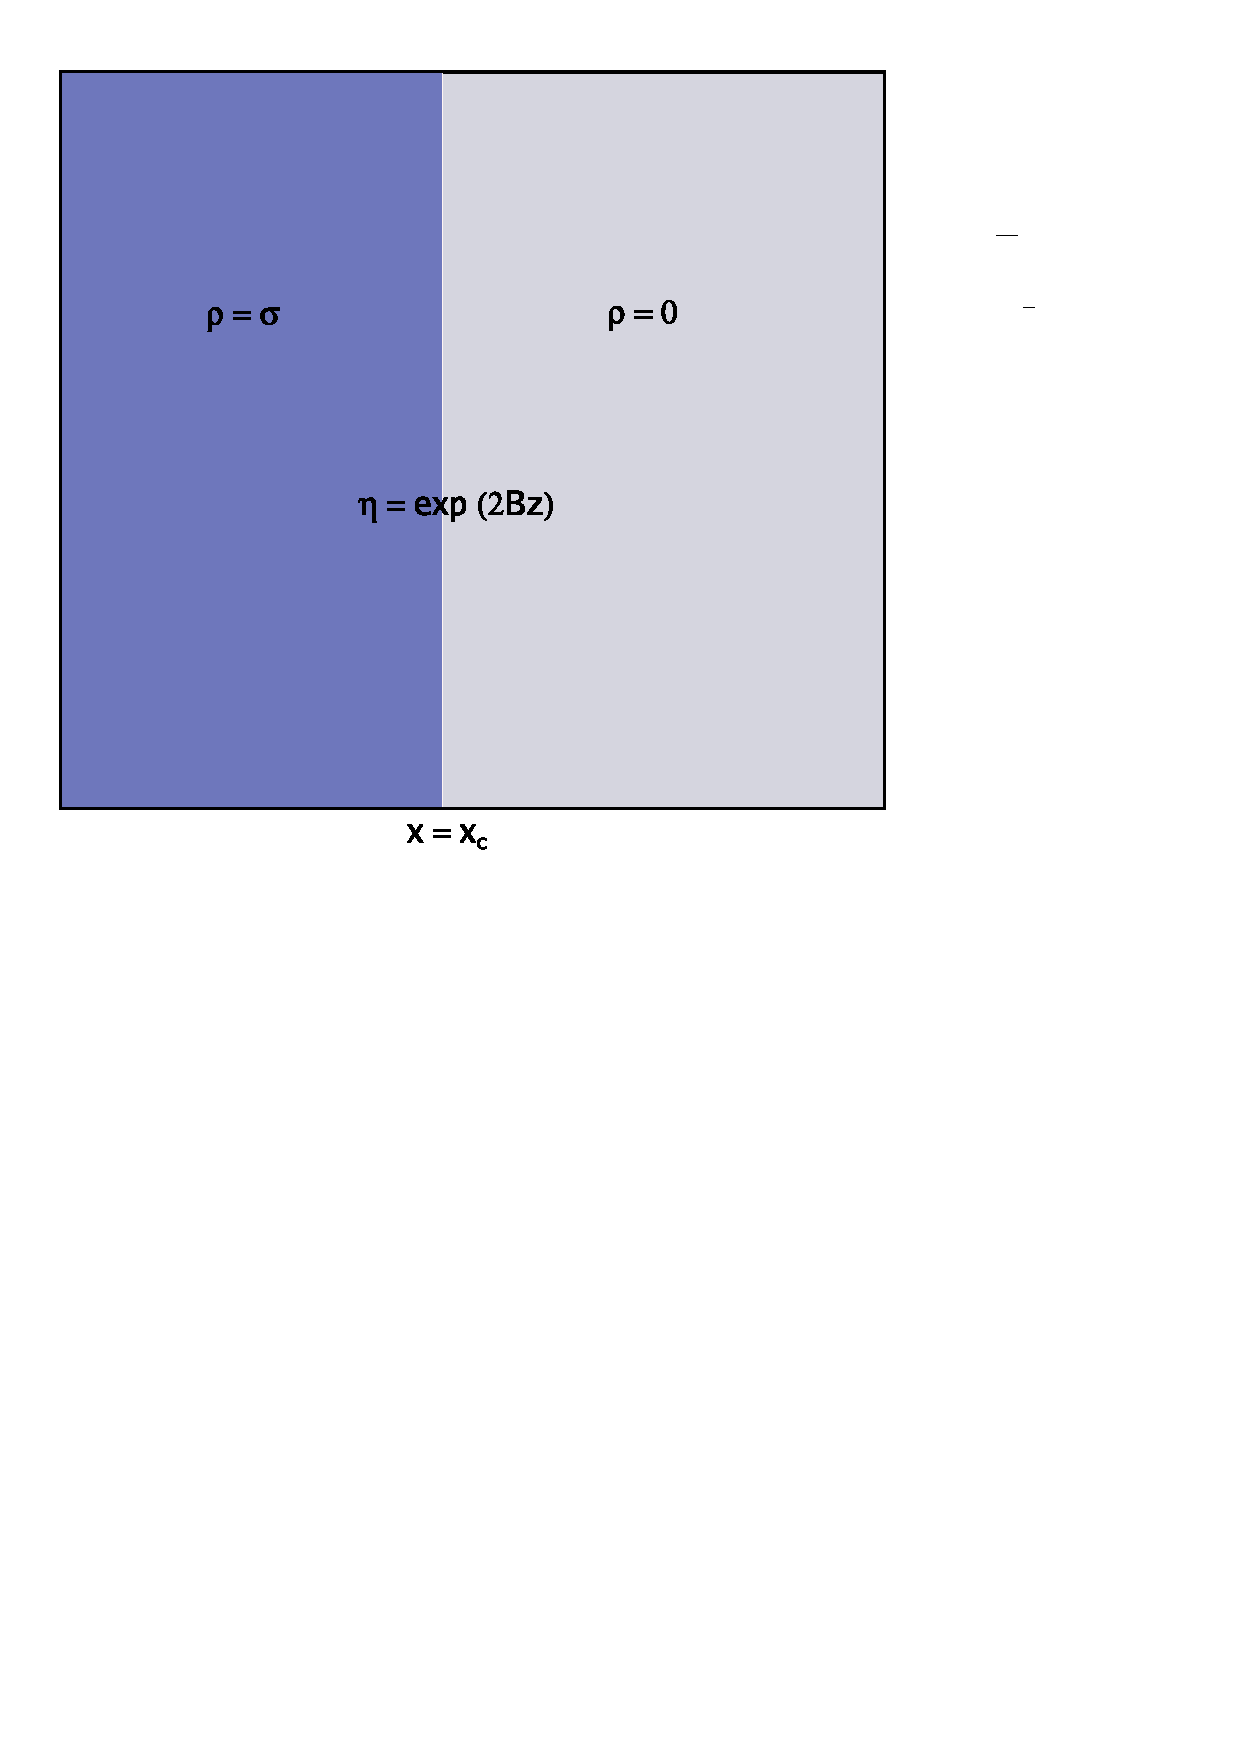
\includegraphics[width=6cm,clip]{../figs/figI}
    \caption[Short caption]{\label{figI} 
      Solution ({\bf SolI}):
      This solution has a column of density $\rho = \sigma$ from $0 < x < x_c$.
      The viscosity varies exponentially in the z direction and is given by
      $\eta = \exp (2 B z)$.
      The boundary conditions are free slip everywhere on the surfaces of the unit box.}
  \end{SCfigure} 
  

